
\documentclass[11pt, a4paper]{article}
\usepackage[utf8]{inputenc}
\usepackage{amsmath, amssymb, amsthm}
\usepackage{geometry}
\usepackage{xcolor}
\usepackage{hyperref}
\usepackage{parskip}
\usepackage{tikz} % Required for drawing diagrams
\usetikzlibrary{arrows.meta, positioning, calc}
\usepackage{caption}

% --- Custom Environments for Pedagogy ---
\usepackage{tcolorbox} % For highlighting key insights
\newtcolorbox{insight}{
    colback=gray!10,
    colframe=black,
    title=\textbf{Pedagogical Insight},
    fonttitle=\bfseries
}

% Geometry settings
\geometry{margin=1in}

% Theorem environments
\newtheorem{definition}{Definition}
\newtheorem{theorem}{Theorem}
\newtheorem{example}{Example}
\newtheorem{remark}{Remark}

% Custom commands
\newcommand{\Q}{\mathbb{Q}}
\newcommand{\Z}{\mathbb{Z}}
\newcommand{\C}{\mathbb{C}}
\newcommand{\Gal}{\text{Gal}}

\title{\textbf{LU003 - An Introduction to Galois Theory}\\ \large Symmetries of Equations and Field Extensions}
\author{Pedagogical Series (Giulio with Gaia)}
\date{Feb 1 2026}

\begin{document}

\maketitle

\begin{abstract}
    This note aims to demystify the foundational definitions of Galois Theory: field extensions, automorphisms, and the Galois group. Rather than stating abstract definitions upfront, we derive them as necessary consequences of algebraic consistency. We begin with the fundamental example of $x^2+1=0$ to illustrate how algebraic symmetries arise from the indistinguishability of roots relative to a base field (e.g., $i$ and $-i$ are merely distinct labels for indistinguishable algebraic twins). Finally, we examine why the Galois group is rarely the full set of permutations, but rather a structure constrained by the ``hidden'' algebraic relations within the field.

    
\end{abstract}

\tableofcontents
\clearpage

\section{The ``Hello World'' of Galois Theory: $\Q(i)$}

Galois theory represents a shift in perspective. In elementary algebra, we ask: \textit{``What are the numbers that solve this equation?''} In Galois theory, we ask: \textit{``How symmetric is the set of solutions? Can we swap them without breaking the arithmetic?''}

Unlike geometric symmetry, which deals with shapes in space, Galois symmetry deals with the algebraic structure of numbers. To make this precise, we define our stage using two fields:
\begin{enumerate}
    \item The \textbf{Base Field} $F = \Q$ (the rational numbers).
    \item The \textbf{Extension Field} $K = \Q(i)$, constructed by adjoining a root of $x^2 + 1 = 0$ to $\Q$. Elements in $K$ are of the form $a + bi$, where $a, b \in \Q$.
\end{enumerate}

\subsection{The Definition of a Symmetry (Automorphism)}

We do not simply swap roots. We look for a structural transformation of the entire field.

\begin{definition}[Field Automorphism]
    An automorphism of an extension $K/\Q$ is a bijective map $\sigma: K \to K$ such that:
    \begin{enumerate}
        \item \textbf{Structure Preservation:} For all $\alpha, \beta \in K$:
        \[ \sigma(\alpha + \beta) = \sigma(\alpha) + \sigma(\beta) \quad \text{and} \quad \sigma(\alpha \cdot \beta) = \sigma(\alpha) \cdot \sigma(\beta) \]
        \item \textbf{Base Fixing:} For all $q \in \Q$, $\sigma(q) = q$.
    \end{enumerate}
\end{definition}


\subsection{Locating the Automorphisms}
Since every element in $\Q(i)$ looks like $a + bi$, and $\sigma$ fixes $a$ and $b$ (because they are rational), the action of $\sigma$ is entirely determined by $\sigma(i)$.

Where can $i$ go? We use the fundamental equation:
\[ i^2 = -1 \]
Apply $\sigma$ to both sides:
\[ \sigma(i^2) = \sigma(-1) \]
Using the homomorphism property and the fact that $-1 \in \Q$:
\[ \sigma(i) \cdot \sigma(i) = -1 \]
\[ (\sigma(i))^2 = -1 \]

\textbf{The Crucial Insight:} $\sigma(i)$ must be a number in our field that \textit{also} squares to $-1$. The roots of $x^2+1$ are $\{i, -i\}$. Thus, there are exactly two possibilities:
\begin{itemize}
    \item \textbf{Case 1 (Identity):} $\sigma(i) = i$. This fixes every element.
    \item \textbf{Case 2 (Conjugation):} $\sigma(i) = -i$. This maps $a+bi \mapsto a-bi$.
\end{itemize}

\begin{center}
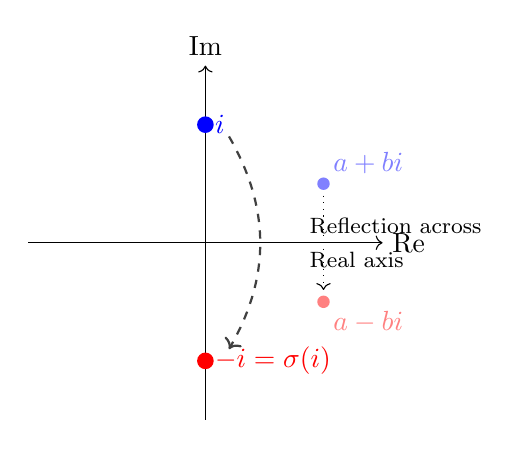
\begin{tikzpicture}[scale=1.5]
    % Axes
    \draw[->] (-1.5,0) -- (1.5,0) node[right] {Re};
    \draw[->] (0,-1.5) -- (0,1.5) node[above] {Im};
    
    % Points
    \fill[blue] (0,1) circle (2pt) node[right] {$i$};
    \fill[red] (0,-1) circle (2pt) node[right] {$-i = \sigma(i)$};
    
    % Reflection Arrow
    \draw[->, dashed, thick, darkgray] (0.2, 0.9) to[bend left] (0.2, -0.9);
    \node at (0.8, 0) [right, align=left] {\footnotesize Reflection across\\ \footnotesize Real axis};
    
    % Generic point
    \fill[blue!50] (1,0.5) circle (1.5pt) node[above right] {$a+bi$};
    \fill[red!50] (1,-0.5) circle (1.5pt) node[below right] {$a-bi$};
    \draw[->, dotted] (1, 0.4) -- (1, -0.4);

\end{tikzpicture}
\captionof{figure}{Visualizing the Automorphism $\sigma(z) = \bar{z}$. Note that the Real axis (Rational numbers) remains fixed, while the Imaginary component flips.}
\end{center}

\subsection{The ``Magic'' of Consistency}
Why is the map $\sigma(i) = -i$ allowed? Does it break the algebra?
Consider the defining relation $i \cdot i = -1$. If we swap $i$ for $-i$, we must ensure the equation still holds.

\begin{center}
\fbox{
\begin{minipage}{0.8\textwidth}
\textbf{Checking the Algebraic "Magic":} \\
We replace $i$ with $-i$. Does the multiplication law hold?
\[ (-i) \cdot (-i) = (-1)(-1)(i \cdot i) = 1 \cdot (-1) = -1 \]
\end{minipage}
}
\end{center}

The swap works precisely because the destination root ($-i$) obeys the same algebraic laws as the source root ($i$). They are "algebraic twins."


\section{The ``Cascade'' of Automorphisms}

A field automorphism is often defined on an infinite set of numbers. However, we do not need to define the mapping for every single number individually. 

\begin{theorem}[Determination by Generators]
    Let $K = \Q(\alpha_1, \dots, \alpha_n)$ be a field extension generated by elements $\alpha_i$. An automorphism $\sigma: K \to K$ fixing $\Q$ is completely determined by the values $\sigma(\alpha_1), \dots, \sigma(\alpha_n)$.
\end{theorem}

\subsection{Proof of the Cascade}
Any element $\gamma \in K$ can be written as a polynomial in the generators with rational coefficients:
\[ \gamma = \sum_{k} c_k (\alpha_1)^{p_1} \dots (\alpha_n)^{p_n} \]
where $c_k \in \Q$.

Applying $\sigma$ to $\gamma$, we use the properties of homomorphism (preservation of $+$ and $\times$) to propagate the map down to the generators:

\begin{align*}
    \sigma(\gamma) &= \sigma\left( \sum_{k} c_k (\alpha_1)^{p_1} \dots (\alpha_n)^{p_n} \right) \\
    &= \sum_{k} \sigma(c_k \cdot (\alpha_1)^{p_1} \dots (\alpha_n)^{p_n}) & (\text{Preservation of Sums}) \\
    &= \sum_{k} \sigma(c_k) \cdot \sigma(\alpha_1)^{p_1} \dots \sigma(\alpha_n)^{p_n} & (\text{Preservation of Products}) \\
    &= \sum_{k} c_k \cdot (\sigma(\alpha_1))^{p_1} \dots (\sigma(\alpha_n))^{p_n} & (\text{Fixing Base Field } \Q)
\end{align*}

\textbf{Conclusion:} The final expression depends \textit{only} on the values of $\sigma(\alpha_i)$. Once the action on the generators is chosen, the action on the entire field is fixed.


\subsection{Algebraic Indistinguishability}
The existence of the automorphism $\sigma(i) = -i$ proves a profound fact about the rational numbers.

\begin{theorem}[Indistinguishability]
    Let $P(x)$ be any polynomial with coefficients in $\Q$. If $P(i) = 0$, then $P(-i) = 0$.
\end{theorem}

\begin{proof}
    Let $P(x) = \sum c_k x^k$ with $c_k \in \Q$. If $P(i) = 0$, apply $\sigma$:
    \[ \sigma\left( \sum c_k i^k \right) = \sigma(0) \]
    Since $\sigma$ fixes $\Q$ and respects powers:
    \[ \sum c_k (\sigma(i))^k = 0 \implies \sum c_k (-i)^k = 0 \implies P(-i) = 0 \]
\end{proof}

There is no algebraic test using rational coefficients that can distinguish $i$ from $-i$.


\subsection{The Counter-Example Analysis}
Consider the polynomial proposed in the discussion:
\[ P(x) = x^3 + i \]
We observe that $i$ is a root: $i^3 + i = -i + i = 0$.
However, if we test $-i$:
\[ P(-i) = (-i)^3 + i = i + i = 2i \neq 0 \]
\textbf{Why did the theorem fail?}
The theorem requires the coefficients of $P(x)$ to be in the base field $\Q$.
Your polynomial has a coefficient $i$, which is in the extension field, not the base field.
\[ i \notin \Q \]

When we apply the automorphism $\sigma$ (conjugation) to the equation $x^3 + i = 0$, we must apply it to the coefficients as well:
\[ \sigma(x^3 + i) = \sigma(0) \]
\[ \sigma(1) \cdot (\sigma(x))^3 + \sigma(i) = 0 \]
Since $\sigma(1)=1$ but $\sigma(i)=-i$, the equation transforms:
\[ x^3 - i = 0 \]
The root $-i$ is a solution to this \textbf{new} equation, not the original one.


\section{Automorphism as Relabeling: the philosophical core of Galois theory}

A field automorphism is effectively a \textbf{relabeling} of the elements that preserves the mathematical truth of the system. 

Consider the field $\Q(i)$. We distinguish the root $i$ from $-i$ by the symbol we write. But algebraically, they are identical:
\begin{itemize}
    \item $i$ is a number that squares to $-1$.
    \item $-i$ is a number that squares to $-1$.
\end{itemize}

If we were to erase every instance of $i$ in a textbook and replace it with $-i$ (and vice-versa), every correct equation would remain correct. The structure $\Q(i)$ does not "know" which one is which. This valid swapping of labels is what we call a non-trivial automorphism.

\subsection{Why $\mathbb{R}$ is Rigid (The Failed Analogy)}

It is natural to ask: can we do this for Real numbers? Can we "relabel" the number line?

 
Consider a mapping where we stretch the number line by a factor $\alpha$:
\[ \sigma(x) = \alpha x \]
If we only cared about \textbf{addition}, this would work. 
\[ \alpha(x+y) = \alpha x + \alpha y \]
This is a valid symmetry of the additive group of real numbers.

However, a Field requires \textbf{multiplication}.
\[ \sigma(x \cdot y) \overset{?}{=} \sigma(x) \cdot \sigma(y) \]
\[ \alpha(xy) \overset{?}{=} (\alpha x)(\alpha y) = \alpha^2 (xy) \]
This forces $\alpha = \alpha^2$, which implies $\alpha = 1$ (Identity) or $\alpha = 0$ (Collapse).
 
Unlike $\Q(i)$, the Real numbers $\mathbb{R}$ have \textbf{no} non-trivial automorphisms. We say the field is "Rigid." 
\begin{itemize}
    \item We cannot swap positive and negative numbers (e.g., $2 \to -2$) because positive numbers have square roots in $\mathbb{R}$, while negative numbers do not. An automorphism must map "squares" to "squares."
    \item We cannot scale numbers ($2 \to 3$) because it breaks the multiplicative structure (as shown above).
\end{itemize}

Galois theory is the study of fields that are "floppy" enough to allow these swaps.


\section{The Core Construction: Equation, Object, Group}
\begin{figure}
    \centering
    \includegraphics[width=1\linewidth]{construction.png}
    \caption{Constructing the Galois Group of an algebraic equation.}
    \label{fig:construction}
\end{figure}
Galois theory represents a shift in perspective. In elementary algebra, we ask: \textit{``What are the numbers that solve this equation?''} In Galois theory, we ask: \textit{``What is the symmetry of the structure generated by these solutions?''}

To answer this, we must formally define the mathematical object we are studying (see Figure~\ref{fig:construction}.

\subsection{Step 1: The Equation}
We begin with a polynomial equation with coefficients in a base field (usually the rational numbers, $\Q$).
\[ x^2 + 1 = 0 \]
This equation has no solutions in our base world $\Q$.

\subsection{Step 2: The Object (The Field Extension)}
To solve the equation, we expand our universe. We create a new field $K$ by adjoining the roots of the polynomial to $\Q$. 
\[ K = \Q(i) = \{ a + bi \mid a, b \in \Q \} \]
This $K$ is our primary mathematical object, called a \textbf{Field Extension}. It contains the roots ($i, -i$) and all their algebraic combinations.

\subsection{Step 3: The Galois Group}
Now we study the symmetry of this object. We look for transformations that scramble the elements of $K$ but preserve its internal algebraic structure.

\begin{definition}[The Galois Group]
    The \textbf{Galois Group} of the extension $K/\Q$, denoted as $\Gal(K/\Q)$, is the set of all field automorphisms $\sigma: K \to K$ that fix the base field $\Q$ pointwise.
    \[ \Gal(K/\Q) = \{ \sigma \in \text{Aut}(K) \mid \sigma(q) = q \text{ for all } q \in \Q \} \]
\end{definition}

In simple terms: The Galois group is the collection of all valid "relabelings" of the extension that leave the rational numbers untouched.


\section{The Galois Group is Not Just Permutations}

One might be tempted to define the Galois group simply as ``the set of all permutations of the roots.'' While the Galois group is always a subgroup of the symmetric group of the roots ($G \subseteq S_n$), it is often strictly smaller.

This occurs because roots often satisfy \textbf{hidden algebraic relations} that must be preserved. A valid automorphism cannot break these relations.

\subsection{Example: The Rigid Structure of Cyclotomic Fields}
Consider the polynomial for the complex 5th roots of unity:
\[ x^4 + x^3 + x^2 + x + 1 = 0 \]
The roots are distinct powers of $\zeta = e^{2\pi i / 5}$:
\[ R = \{ \zeta, \zeta^2, \zeta^3, \zeta^4 \} \]

The set of roots has size 4. The full group of permutations ($S_4$) has $4! = 24$ elements. However, the Galois group has only \textbf{4 elements}.

\begin{center}
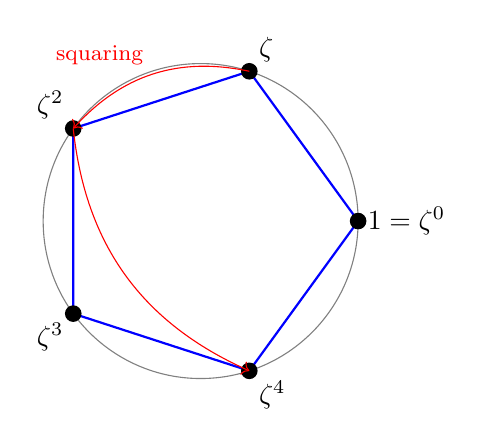
\begin{tikzpicture}[scale=2]
    % Circle
    \draw[gray, thin] (0,0) circle (1cm);
    
    % Vertices of the Pentagon
    \foreach \i in {0,1,2,3,4} {
        \coordinate (P\i) at ({cos(72*\i)}, {sin(72*\i)});
    }
    
    % Draw Pentagon
    \draw[thick, blue] (P0) -- (P1) -- (P2) -- (P3) -- (P4) -- cycle;
    
    % Nodes
    \fill[black] (P0) circle (1.5pt) node[right] {$1 = \zeta^0$};
    \fill[black] (P1) circle (1.5pt) node[above right] {$\zeta$};
    \fill[black] (P2) circle (1.5pt) node[above left] {$\zeta^2$};
    \fill[black] (P3) circle (1.5pt) node[below left] {$\zeta^3$};
    \fill[black] (P4) circle (1.5pt) node[below right] {$\zeta^4$};
    
    % Arrow showing structure
    \draw[->, red, bend right] (P1) to node[auto, swap] {\footnotesize squaring} (P2);
    \draw[->, red, bend right] (P2) to (P4);
    
\end{tikzpicture}
\captionof{figure}{The "Rigid" Structure. The roots form a regular pentagon. More importantly, they are powers of each other. If you move $\zeta$, you drag $\zeta^2$ (which is $\zeta \cdot \zeta$) with it.}
\end{center}

\subsubsection*{Why can't we just swap any two roots?}
Suppose we try to construct a permutation $\tau$ that swaps $\zeta$ and $\zeta^2$ but leaves $\zeta^3$ fixed.
\[ \tau(\zeta) = \zeta^2, \quad \tau(\zeta^2) = \zeta, \quad \tau(\zeta^3) = \zeta^3 \]
This is a valid permutation of the set $R$. However, let us check if it is a valid field automorphism.

In the field, $\zeta^2$ is algebraically related to $\zeta$ by the squaring operation:
\[ \zeta^2 = \zeta \cdot \zeta \]
A valid automorphism $\tau$ must respect this multiplication:
\[ \tau(\zeta^2) = \tau(\zeta \cdot \zeta) = \tau(\zeta) \cdot \tau(\zeta) \]
Substitute our proposed values:
\[ \text{LHS: } \tau(\zeta^2) = \zeta \]
\[ \text{RHS: } \tau(\zeta) \cdot \tau(\zeta) = \zeta^2 \cdot \zeta^2 = \zeta^4 \]
\[ \zeta \neq \zeta^4 \]

The relation is broken. The roots are ``locked'' together by the exponential relation. Once you decide where $\zeta$ goes, the destination of $\zeta^2, \zeta^3,$ and $\zeta^4$ is mathematically forced. This rigidity drastically reduces the size of the Galois group.

\subsection{Summary}
The Galois group measures the ``ambiguity'' of the roots relative to the base field.
\begin{itemize}
    \item It is the group of automorphisms of the splitting field that fix the base field.
    \item It is a subgroup of the permutations of the roots.
    \item It is the full symmetric group ($S_n$) only when there are no algebraic relations between the roots other than the polynomial equation itself.
\end{itemize}

\section{Closing: The Philosophy of Mathematical Structure}

Mathematics is often mischaracterized as the study of calculations. More accurately, it is the study of \textit{structures}. A mathematical structure is not merely a collection of objects; it is a rigorous "environment" or "landscape" defined by specific constraints.

Much of modern mathematics studies \emph{structures}: collections of objects equipped with specified operations and relations, constrained by axioms. The axioms are not mere restrictions; they are what make reasoning \emph{stable} and \emph{transportable} across contexts.


\begin{figure}[t]
    \centering
    \includegraphics[width=1\linewidth]{structure.png}
    \caption{A pedagogical illustration visualized as a chalkboard diagram, explaining the concept of mathematical structure in the context of a field extension, such as $L = \mathbb{Q}(i)$ over the base field $K = \mathbb{Q}$. The base field is depicted as a solid foundation, upon which a rigid framework of "Structural Constraints" (axioms and rules) is built, supporting the extended field $L$. This constrained environment ensures "Consistency," as shown by two different calculation paths (A and B) converging to the same result. The diagram also illustrates "Symmetry" (an automorphism) as a transformation that swaps indistinguishable roots while leaving the underlying structure invariant.}
    \label{fig:structure}
\end{figure}

\subsection{Structure as Constraint}
To build a structure is to impose rules. When we define a Group, a Ring, or a Field, we are essentially saying: "You cannot move arbitrarily; you must move according to these laws." 

Paradoxically, these constraints are what give mathematics its power. Because we are moving in a constrained world, we gain \textbf{consistency}.
\begin{itemize}
    \item \textbf{Path Independence:} In a structured world, if you start at point $A$ and apply valid operations to reach point $B$, the specific path you took often matters less than the rules you followed. 
    \item \textbf{Predictability:} If we calculate $(a+b)^2$ in the integers, or in the real numbers, or in a complex field, the result is always $a^2 + 2ab + b^2$. The \textit{structural rules} (distributivity and commutativity) guarantee this consistency across different contexts.
\end{itemize}

\begin{insight}
    \textbf{Structure ensures Semantic Consistency.} \\
    You can perform a calculation in different ways—grouping terms differently (associativity) or ordering them differently (commutativity)—and arrive at the exact same endpoint. This is only possible because the structure is "rigid." It holds its shape under calculation. \\

    Axioms license rewrites (rebracketing, expansion, reordering when permitted) that preserve denotation. “Different-looking” derivations converge because they are constrained by the same invariants.
\end{insight}

\subsection{Extending Structures: The Case of $\mathbb{Q}(i)$}

This perspective is crucial when we discuss \textbf{field extensions}. When we extend a field, we are expanding our "landscape," but we demand that the new landscape respects the structural integrity of the old one.

Consider the extension of the rational numbers $\Q$ by the imaginary unit $i$, denoted as $\Q(i)$.
\[
    \Q(i) = \{ a + bi \mid a, b \in \Q \}
\]
We are not simply throwing $i$ into a bag with rational numbers. We are forcing $i$ to submit to the pre-existing arithmetic structure of $\Q$.
\begin{itemize}
    \item We demand that multiplication remains distributive.
    \item We demand that addition remains commutative.
\end{itemize}

Because of these constraints, the behavior of every new element is pre-determined. For example, the product of $(1+i)$ and $(1-i)$ is not arbitrary; the structure forces it to be $2$. The "grid" of numbers has expanded, but the "lines of logic" connecting them remain straight and unbroken.

\subsection{From Structure to Symmetry}

Finally, structure gives rise to \textit{symmetry}. In a purely chaotic set with no structure, "symmetry" is meaningless because there is no shape to preserve. Symmetry is, by definition, a transformation that leaves the underlying structure invariant.

In our example of $\Q(i)$, the structure is defined by the rational numbers and the property that $i^2 = -1$. 
\begin{itemize}
    \item Notice that $(-i)^2 = -1$ as well.
    \item From the perspective of the structure $\Q$, the elements $i$ and $-i$ are indistinguishable. They play the exact same structural role.
\end{itemize}

This structural ambiguity allows us to swap $i$ and $-i$ without breaking the arithmetic. This swap is a \textbf{symmetry} (specifically, an automorphism). 




Structure thus gives rise to \emph{symmetry} in the precise sense of \emph{structure-preserving maps}. In field theory, the relevant symmetries are \textbf{field automorphisms} that fix the base field pointwise.

% In $\mathbb{Q}(i)/\mathbb{Q}$, an automorphism $\sigma$ must fix every rational number, and it must send $i$ to another element satisfying the same defining constraints. Concretely, $i$ is a root of its minimal polynomial over $\mathbb{Q}$,
% \[
% x^2+1,
% \]
% so any $\mathbb{Q}$-automorphism must send $i$ to another root of $x^2+1$, i.e., to $i$ or $-i$. Thus there are exactly two symmetries:
% \[
% \sigma(i)=i \quad\text{or}\quad \sigma(i)=-i,
% \]
% giving $\mathrm{Gal}(\mathbb{Q}(i)/\mathbb{Q})\cong C_2$.

\begin{insight}
    \textbf{Symmetry is the Shadow of Structure.} \\
    The more rigid and constrained the structure, the more meaningful the symmetries become. In Galois Theory, we study field extensions by analyzing these symmetries. We ask: "What are the ways we can move around inside this structure without breaking the rules?" \\

    Automorphisms are precisely the self-maps that preserve all axioms and defining relations. Studying an extension via its automorphisms is the core move of Galois theory: classify what can change without breaking the rules.
\end{insight}





\section{Algorithmic Structure and Galois Symmetry: the Example of $\mathbb{Q}(i)$}
\label{sec:ait-galois-qi}

A useful way to connect \emph{algorithmic information} (AIT) and \emph{Galois theory} is to treat a mathematical structure as something generated by a concise specification (a ``short program''), and to view \emph{symmetry} as the residual ambiguity left once the specification has fixed all invariants it can.

\subsection{A short generative description of the extension}
The field $\mathbb{Q}(i)$ can be defined by a minimal algorithmic specification:
\begin{quote}
Start with $\mathbb{Q}$ and adjoin an element $x$ subject to the single constraint $x^2+1=0$.
\end{quote}
Formally, this construction is captured by the quotient
\begin{equation}
\mathbb{Q}(i)\ \cong\ \mathbb{Q}[x]/(x^2+1),
\label{eq:Qi-quotient}
\end{equation}
where the coset $[x]$ plays the role of $i$, and every element has a unique representative $a+bx$ with $a,b\in\mathbb{Q}$ (reduction modulo $x^2+1$). This is a standard instance of the general fact that adjoining an algebraic element $\alpha$ with minimal polynomial $m_\alpha(x)$ yields an isomorphic field $F(\alpha)\cong F[x]/(m_\alpha(x))$ \cite{MilneFT,ArtinGalois71}.

From an AIT/MDL viewpoint, Eq.~\eqref{eq:Qi-quotient} emphasizes that the extension is specified by a \emph{small description}: ``the base field $\mathbb{Q}$, plus a single polynomial constraint $x^2+1=0$, plus the canonical quotient construction.'' In this sense, the \emph{regularity} defining $\mathbb{Q}(i)$ is precisely what makes the structure compressible in the Kolmogorov/MDL sense \cite{Kolmogorov65,Rissanen78}.


\begin{figure} [t]
    \centering
    \includegraphics[width=1\linewidth]{compression.png}
    \caption{\textbf{The Algorithmic Origins of Symmetry.} 
This diagram illustrates the synthesis of Algorithmic Information Theory (AIT) and Galois Theory using the extension $\mathbb{Q}(i)$. 
\textbf{(Left)} The minimal polynomial $P(x) = x^2+1$ is viewed as a "generating program" with low Kolmogorov complexity. This short code completely describes the structure of the extension. 
\textbf{(Center)} Because the program specifies a relationship ($x^2 = -1$) rather than unique identities, it leads to "algorithmic indistinguishability" between the solutions.
\textbf{(Right)} This indistinguishability manifests as a symmetry (automorphism) in the complex plane, where swapping the roots $i$ and $-i$ leaves the underlying algorithmic structure invariant.}
    \label{fig:compression}
\end{figure}

\subsection{Symmetry as residual ambiguity compatible with the specification}
Once the extension is fixed by its defining constraint, the admissible symmetries are exactly those transformations that preserve \emph{all} structure---i.e., field automorphisms fixing the base field pointwise. In $\mathbb{Q}(i)/\mathbb{Q}$, any $\sigma\in\mathrm{Gal}(\mathbb{Q}(i)/\mathbb{Q})$ must fix $\mathbb{Q}$ and send $i$ to another element satisfying the same minimal polynomial $x^2+1$. Since the roots are $\{i,-i\}$, there are exactly two possibilities:
\begin{equation}
\sigma(i)=i\quad\text{or}\quad \sigma(i)=-i,
\end{equation}
so
\begin{equation}
\mathrm{Gal}(\mathbb{Q}(i)/\mathbb{Q})\ \cong\ C_2.
\label{eq:gal-qi}
\end{equation}
Thus, the sole nontrivial symmetry is the swap $i\mapsto -i$ (complex conjugation restricted to $\mathbb{Q}(i)$) \cite{ArtinGalois71,MilneFT}.

\subsection{An AIT reading: ``one bit'' of unresolved choice}
The defining ``program'' for $\mathbb{Q}(i)$ specifies the extension \emph{up to} the choice of which root is named as the generator: the constraint $x^2+1=0$ does not distinguish $i$ from $-i$. This leftover indistinguishability is exactly the Galois symmetry in Eq.~\eqref{eq:gal-qi}. In this toy example, the size of the symmetry group corresponds to a literal ``one-bit'' ambiguity:
\begin{equation}
\log_2 \big|\mathrm{Gal}(\mathbb{Q}(i)/\mathbb{Q})\big|=\log_2 2=1.
\end{equation}
Interpretationally: given the concise generative description (Eq.~\eqref{eq:Qi-quotient}), specifying a particular identification of the adjoined element requires one additional bit (choose the $+$ or $-$ root). In this sense, \emph{Galois symmetry measures the degrees of freedom that remain after the structural constraints have fixed all invariants they can}.

\paragraph{Takeaway.}
Structure can be viewed as a compressive, algorithmic specification (constraints + canonical construction), while symmetry is the ``shadow'' of that specification: the transformations that preserve all constraints, equivalently the residual ambiguity not resolved by the description. The extension $\mathbb{Q}(i)/\mathbb{Q}$ provides a minimal illustration: a short description generates the structure, and the single surviving ambiguity manifests as the nontrivial Galois automorphism $i\mapsto -i$.




% \section{The Philosophy of Mathematical Structure}

% Mathematics is sometimes caricatured as the art of calculation. More accurately, much of modern mathematics studies \emph{structures}: collections of objects equipped with specified operations and relations, constrained by axioms. The axioms are not mere restrictions; they are what make reasoning \emph{stable} and \emph{transportable} across contexts.

% \subsection{Structure as Constraint (and as Invariance)}
% To define a group, ring, or field is to specify which transformations and manipulations are \emph{legal}. The payoff is that legality is \emph{invariant}: any two expressions related by the axioms represent the same element.

% \begin{itemize}
%     \item \textbf{Well-definedness (invariance under rewriting):} If you start with an expression and rewrite it using valid identities (associativity, distributivity, etc.), the final value does not depend on superficial choices such as parenthesization.
%     \item \textbf{Predictability from axioms:} In any \emph{commutative} ring/field,
%     \[
%         (a+b)^2 = a^2 + 2ab + b^2,
%     \]
%     because distributivity expands $(a+b)(a+b)$ and commutativity identifies $ab=ba$. In a noncommutative ring, the structurally correct identity is
%     \[
%         (a+b)^2 = a^2 + ab + ba + b^2.
%     \]
% \end{itemize}

% \begin{insight}
%     \textbf{Structure ensures invariance of meaning.}\\
%     Axioms license rewrites (rebracketing, expansion, reordering when permitted) that preserve denotation. “Different-looking” derivations converge because they are constrained by the same invariants.
% \end{insight}

% \subsection{Extending Structures: The Case of $\mathbb{Q}(i)$}

% This viewpoint is crucial for \textbf{field extensions}. When we extend a field, we enlarge the domain of discourse while requiring that the original arithmetic remains intact.

% Adjoin a symbol $i$ to $\mathbb{Q}$ subject to the single relation $i^2=-1$. Formally, one clean construction is
% \[
% \mathbb{Q}(i)\ \cong\ \mathbb{Q}[x]/(x^2+1),
% \]
% so every element has a unique representative of the form $a+bi$ with $a,b\in\mathbb{Q}$ and multiplication is polynomial multiplication modulo $x^2+1$.

% \begin{itemize}
%     \item Distributivity, associativity, and commutativity of addition are inherited from $\mathbb{Q}$.
%     \item The relation $i^2=-1$ fixes how new products reduce.
% \end{itemize}

% For example, the structure forces
% \[
% (1+i)(1-i) = 1 - i^2 = 2.
% \]
% The “grid” has expanded, but arithmetic remains coherent because it is defined by inherited axioms plus the defining relation.

% \subsection{From Structure to Symmetry}

% Structure gives rise to \emph{symmetry} in the precise sense of \emph{structure-preserving maps}. In field theory, the relevant symmetries are \textbf{field automorphisms} that fix the base field pointwise.

% In $\mathbb{Q}(i)/\mathbb{Q}$, an automorphism $\sigma$ must fix every rational number, and it must send $i$ to another element satisfying the same defining constraints. Concretely, $i$ is a root of its minimal polynomial over $\mathbb{Q}$,
% \[
% x^2+1,
% \]
% so any $\mathbb{Q}$-automorphism must send $i$ to another root of $x^2+1$, i.e., to $i$ or $-i$. Thus there are exactly two symmetries:
% \[
% \sigma(i)=i \quad\text{or}\quad \sigma(i)=-i,
% \]
% giving $\mathrm{Gal}(\mathbb{Q}(i)/\mathbb{Q})\cong C_2$.

% \begin{insight}
%     \textbf{Symmetry is the residue of freedom left by constraints.}\\
%     Automorphisms are precisely the self-maps that preserve all axioms and defining relations. Studying an extension via its automorphisms is the core move of Galois theory: classify what can change without breaking the rules.
% \end{insight}



% --- Bibitems for the AIT–Galois section ---
\begin{thebibliography}{99}
\bibitem{MilneFT}
J.~S.~Milne,
\newblock \emph{Fields and Galois Theory} (course notes, v4.60, Sept.~2018).
\newblock Available at:
\href{https://www.jmilne.org/math/CourseNotes/FT.pdf}{https://www.jmilne.org/math/CourseNotes/FT.pdf}.

% \bibitem{ArtinGalois42}
% E.~Artin,
% \newblock \emph{Galois Theory: Lectures Delivered at the University of Notre Dame},
% \newblock Notre Dame Mathematical Lectures, No.~2, University of Notre Dame, 1942.
% \newblock Available at:
% \href{https://projecteuclid.org/ebooks/notre-dame-mathematical-lectures/Galois-Theory/toc/ndml/1175197001}{Project Euclid (NDML)}.

% (Optional alternate edition, if you prefer citing the revised later printing)
\bibitem{ArtinGalois71}
E.~Artin,
\newblock \emph{Galois Theory: Lectures Delivered at the University of Notre Dame} (rev. ed.),
\newblock edited by A.~N.~Milgram, Notre Dame Mathematical Lectures, No.~2, 1971.
\newblock Available at:
\href{https://projecteuclid.org/ebooks/notre-dame-mathematical-lectures/Galois-Theory/toc/ndml/1175197041}{Project Euclid (NDML)}.

\bibitem{Kolmogorov65}
A.~N.~Kolmogorov,
\newblock ``Three approaches to the definition of the concept `quantity of information',''
\newblock \emph{Problemy Peredachi Informatsii} \textbf{1}(1): 3--11, 1965.
\newblock Accessible PDF:
\href{https://alexander.shen.free.fr/library/Kolmogorov65_Three-Approaches-to-Information.pdf}{https://alexander.shen.free.fr/library/Kolmogorov65\_Three-Approaches-to-Information.pdf}.
\newblock (Reprint/translation: \emph{International Journal of Computer Mathematics} \textbf{2}(1--4): 157--168, 1968,
DOI \href{https://doi.org/10.1080/00207166808803030}{10.1080/00207166808803030}.)

\bibitem{Rissanen78}
J.~Rissanen,
\newblock ``Modeling by shortest data description,''
\newblock \emph{Automatica} \textbf{14}(5): 465--471, 1978.
\newblock DOI \href{https://doi.org/10.1016/0005-1098(78)90005-5}{10.1016/0005-1098(78)90005-5}.
\end{thebibliography}
\end{document}
